\documentclass{beamer}
\usepackage[utf8]{inputenc}
\usepackage[german]{babel}
\usepackage{graphicx}
\usepackage{tikz}
\usepackage{xcolor}
\usepackage[export]{adjustbox}
\usepackage{subfig}
\usepackage{graphbox}
\usepackage[autostyle=true,german=quotes]{csquotes}
\MakeOuterQuote{"}
\begin{document}


\setbeamertemplate{navigation symbols}{}
\addtobeamertemplate{navigation symbols}{}{%
    \usebeamerfont{footline}%
    \usebeamercolor[fg]{footline}%
    \hspace{1em}%
    \insertframenumber/\inserttotalframenumber
}

\usebackgroundtemplate{
  \tikz\node[opacity=0.3]
  {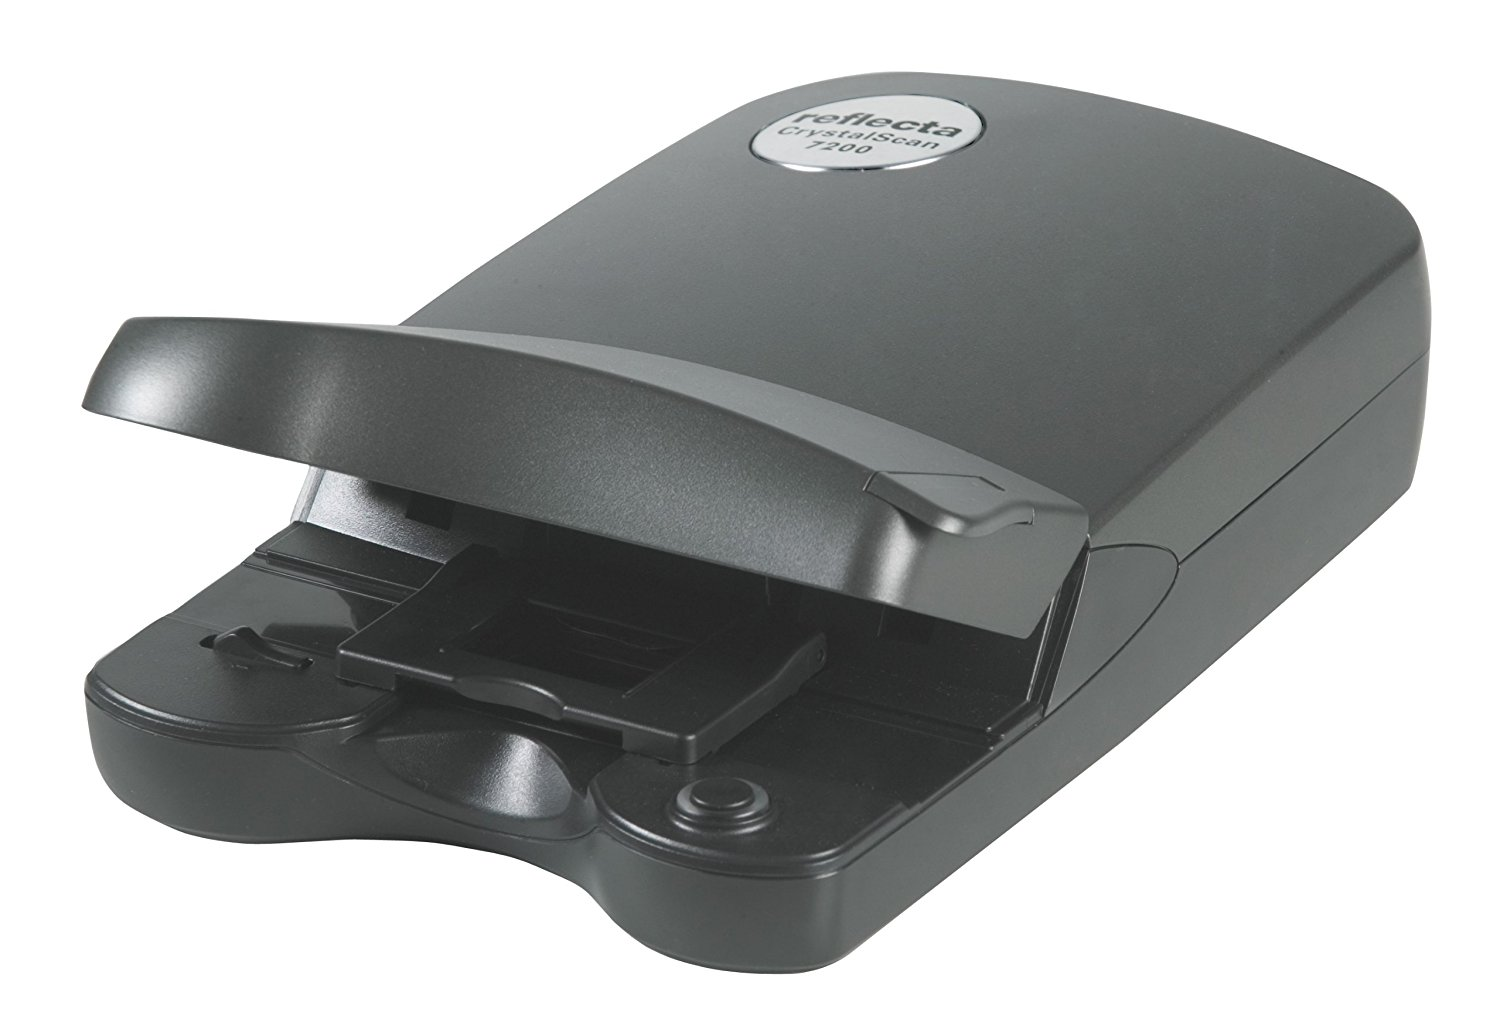
\includegraphics[height=\paperheight,width=\paperwidth]
  {images/presentation/the_scanner.jpg}};
}

\title{Entwicklung eines Treibers für einen Filmscanner mittels USB-Sniffing und Reverse Engineering}
\author{Hugo Platzer}
\date{}

\frame{\titlepage}

\usebackgroundtemplate{}
\frame{\frametitle{Reflecta CrystalScan 7200}
  \begin{itemize}
    \item Zum Digitalisieren von Kleinbilddias / -negativen
    \begin{figure}[H]
      \subfloat{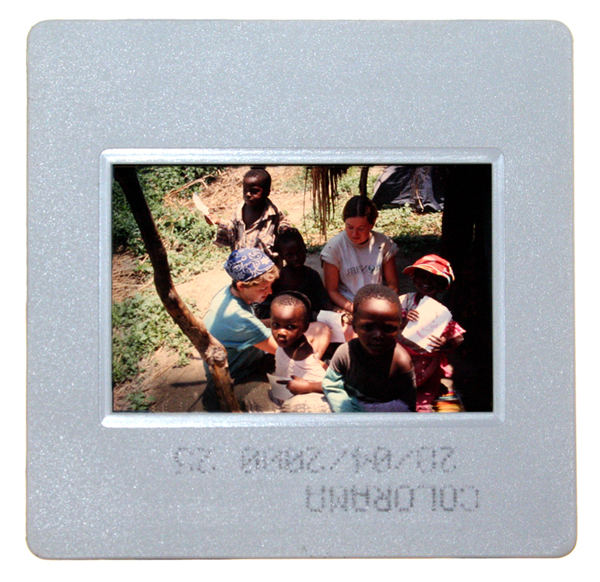
\includegraphics[height=1.5cm]{images/presentation/film_pos.jpg} }
      \quad
      \subfloat{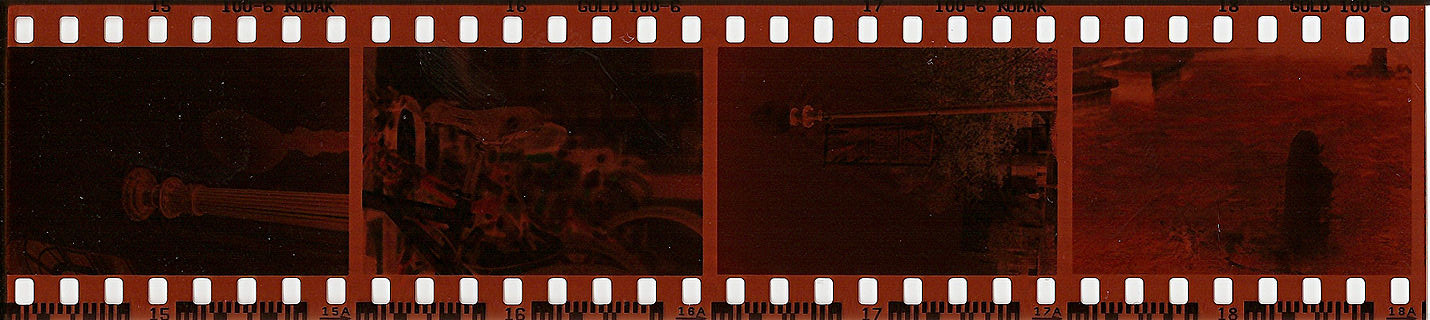
\includegraphics[height=1.5cm]{images/presentation/film_neg.jpg} }
      \hspace{\fill}
    \end{figure}
    \item Per USB verbunden
    \item Software nur für Windows / Mac
    \item Versuch, einen Linux-Treiber zu entwickeln ohne entsprechende
          Dokumentation
  \end{itemize}
}

\frame{\frametitle{Reverse Engineering}
  \begin{itemize}
    \item Prozess des "Engineering" (von der Spezifikation zum Produkt) in
          umgekehrter Richtung
    \item Versuch, aus für den Konsumenten verfügbaren Daten (Firmware, Software,
          Mitlauschen an Schnittstellen) Protokolle zu rekonstruieren
    \item Rechtliche Grauzone
    \item Um Einverständnis gebeten: Hersteller war kooperativ
  \end{itemize}
}

\frame{\frametitle{Der USB-Standard}
  \begin{itemize}
    \item ein Anschluss für alle Klassen von Geräten
    \item Alle Kommunikation geht vom Host aus
    \item Übertragung in Paketen {\tt >} Transactions {\tt >} Transfers
    \item ein Gerät hat oft mehrere Kanäle (Endpoints)
    \item Control-Endpoint
    \begin{itemize}
      \item besitzt jedes Gerät, dient zur Steuerung
      \item definierte Nachrichtenform mit Parametern und Zusatzdaten
      \item Standard Requests: Vom USB-Standard vorgeschriebene Basisfunktionen
      \item Vendor-specific Requests: Herstellerspezifische Zusatzfunktionen,
            undokumentiert
    \end{itemize}
    \item Bulk-Endpoint
    \begin{itemize}
      \item für große Datenmengen (Dateien, Bilddaten)
      \item Bytestrom ohne Struktur
    \end{itemize}
  \end{itemize}
}

\frame{\frametitle{USB-Sniffing}
  \begin{itemize}
    \item Mitschneiden der Kommunikation zwischen Gerät und Windows-Software
    \item Kernelmodul {\tt usbmon}
    \begin{itemize}
      \item Zugang zu vom Linux-Kernel abgearbeiteten USB-Transfers
      \item Schwierigkeiten bei langer Payload
    \end{itemize}
    \item Wireshark
    \begin{itemize}
      \item Netzwerk-Sniffer, der sich auch für USB eignet
      \item sowohl zur Aufzeichnung als auch Analyse
      \item flexibel anpassbare Oberfläche
    \end{itemize}
    \item VirtualBox
    \begin{itemize}
      \item Windows in virtueller Maschine unter Linux ausführen
      \item USB-Passthrough gibt Windows Zugang zum Scanner
    \end{itemize}
  \end{itemize}
}

\frame{\frametitle{Wireshark}
  \noindent\makebox[\textwidth]{
    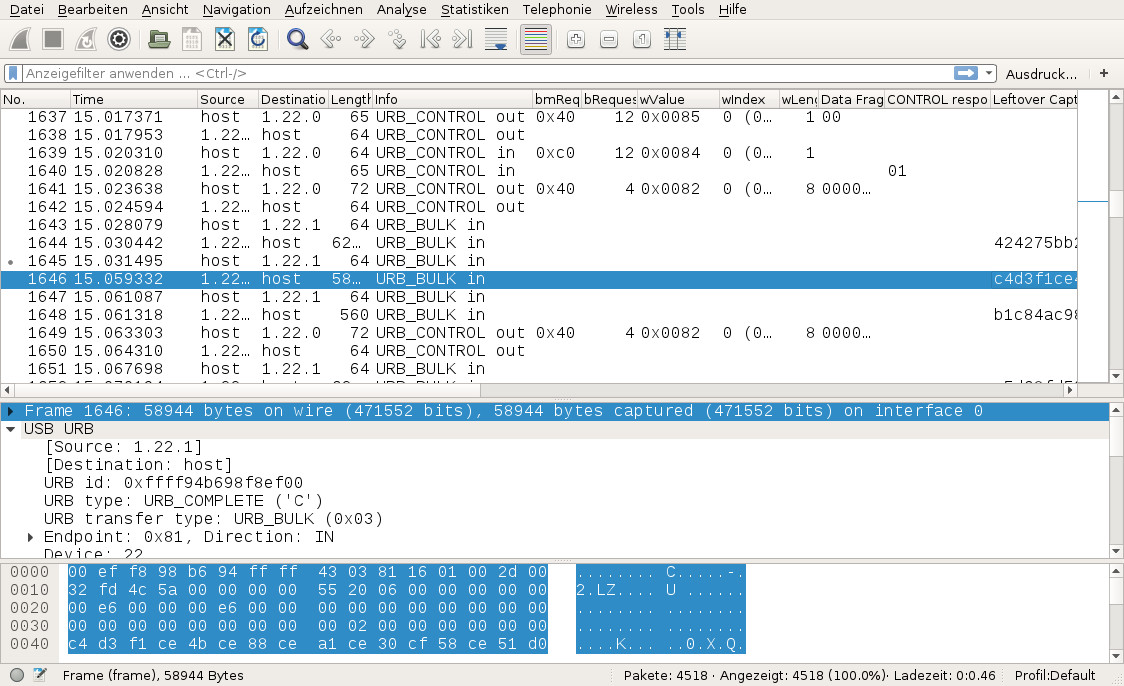
\includegraphics[width=\paperwidth]{images/presentation/wireshark.jpg}
  }
}

\frame{\frametitle{usbmon: unvollständige Payload}
  \begin{itemize}
    \item Bei großen Paketen wird Payload nach 61440 Bytes abgeschnitten
    \item visuell: Risse im rekonstruierten Bild
      \begin{figure}[H]
        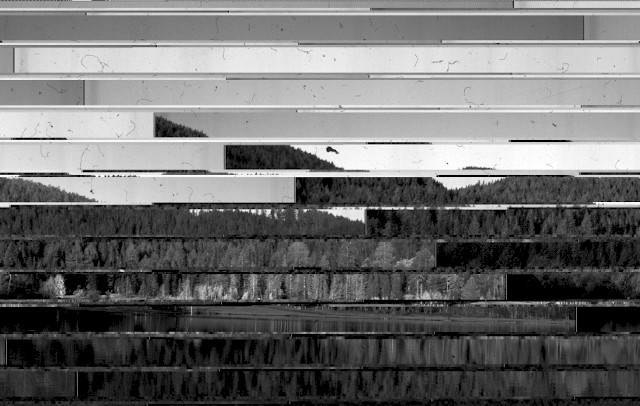
\includegraphics[height=4cm,left]{images/reconstruct_missing.jpg}
      \end{figure}
    \item gelöst durch einfachen Kernel-Patch
    
      {\small \tt if (length >= rp->b\_size \textcolor{red}{/ 5})
           length = rp->b\_size \textcolor{red}{/ 5};}
  \end{itemize}
}


\frame{\frametitle{Analyse der Aufzeichnung}
  \begin{itemize}
    \item Versuche, das übertragene Bild aus Aufzeichnung zu rekonstruieren
    \item Parsen des .pcap-File mit {\tt tshark}
    \begin{itemize}
      \item in Wireshark alle Protokolle außer USB deaktivieren!
    \end{itemize}
    \item Bilddaten werden über große Bulk-Transfers übertragen
    \item zeilenweise 16-bit Little Endian Pixelwerte
    \begin{figure}[H]
      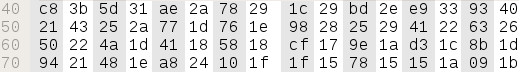
\includegraphics[height=1.3cm,left]{images/extract_sniff2.jpg}
    \end{figure}
    \item eingehende Bytes am Bulk-Endpoint sammeln, dann weiterverarbeiten:
    \begin{itemize}
      \item Offsets
      \item $16 \to 8$ Bit
      \item In Zeilen gruppieren
      \item usw.
    \end{itemize}
  \end{itemize}
}


\frame{\frametitle{Rekonstruktion des Bildes}
    \noindent\makebox[\textwidth]{
    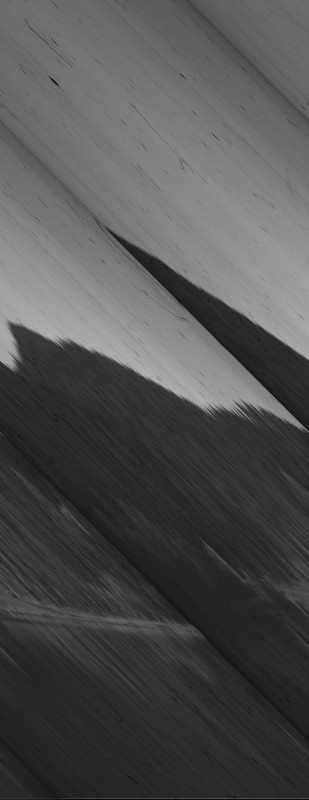
\includegraphics[height=4cm]{images/presentation/extract_raw.jpg}
    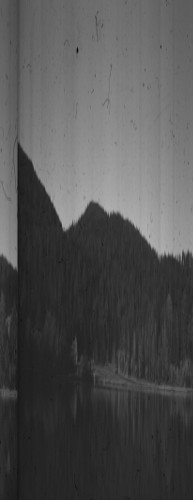
\includegraphics[height=4cm]{images/extract_3.jpg}
    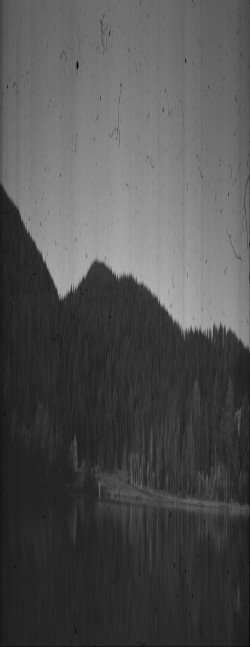
\includegraphics[height=4cm]{images/extract_2.jpg}
    
\includegraphics[height=2cm]{images/extract_5.jpg}
    }
    \\ \vspace{0.1cm}
    \noindent\makebox[\textwidth]{
    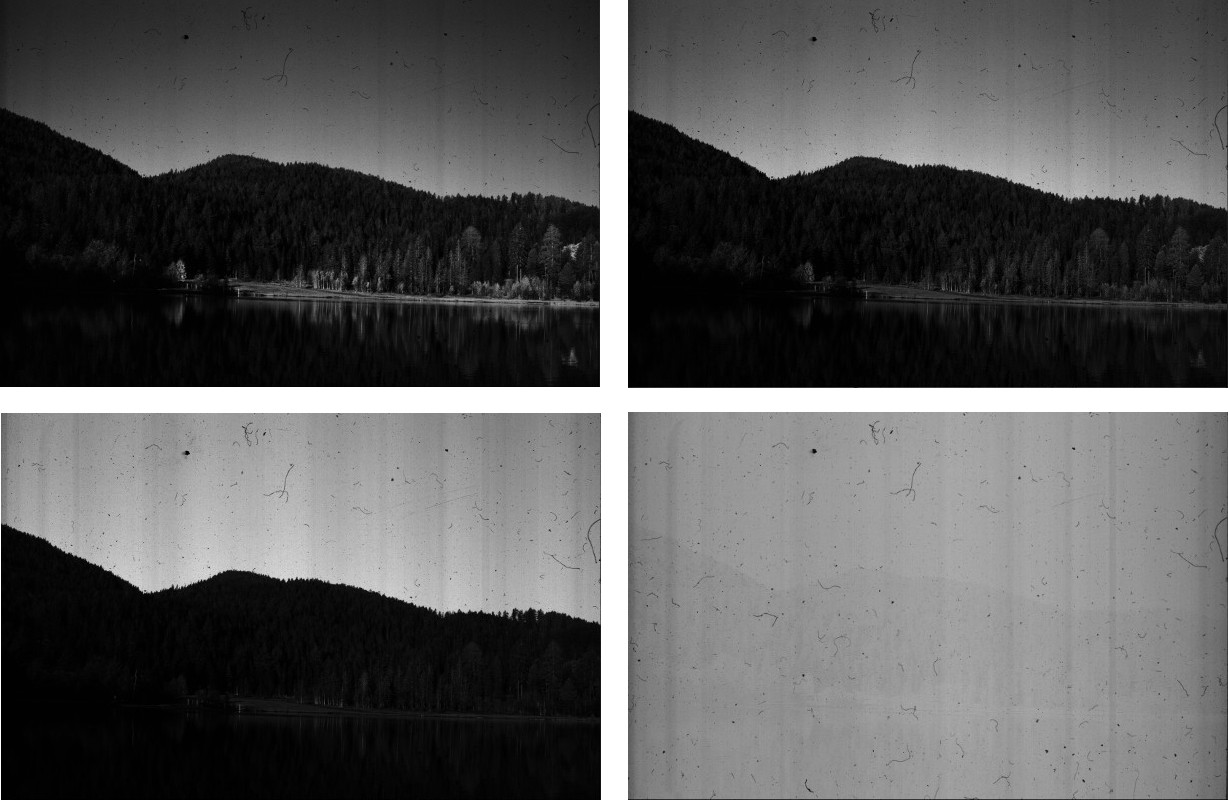
\includegraphics[height=2.5cm]{images/presentation/extract_channels.jpg}
    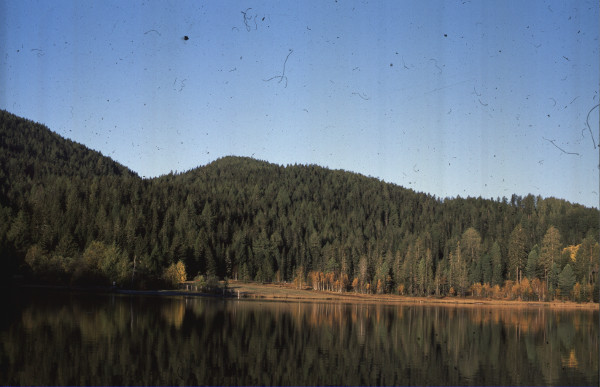
\includegraphics[height=2.5cm]{images/extract_7a.jpg}
    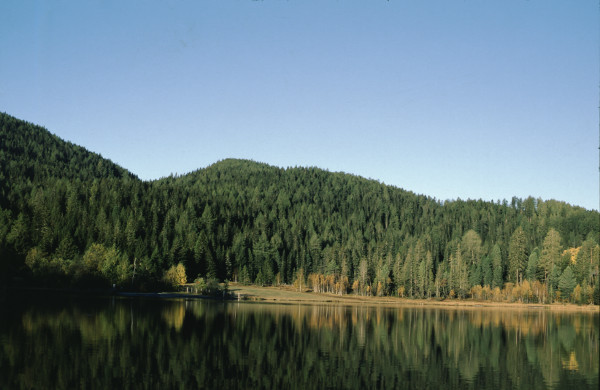
\includegraphics[height=2.5cm]{images/extract_7b.jpg}
    }
}

\frame{\frametitle{Ansteuern des Scanners}
  \begin{itemize}
    \item {\tt PyUSB} - basiert
    \item Grundidee: aufgezeichnete Befehlsfolge zum Gerät wieder abspielen, eingehende Daten speichern
    \item viele Muster in der Kommunikation erkennbar
    \begin{figure}[H]
      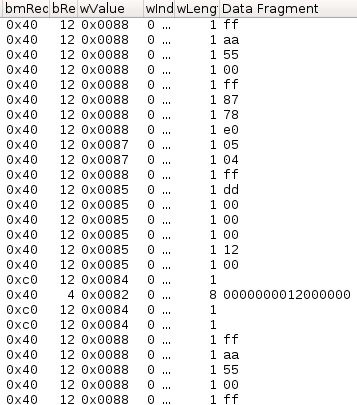
\includegraphics[height=6cm,left]{images/presentation/sniff_pattern.jpg}
    \end{figure}
  \end{itemize}
}

\frame{\frametitle{Zeitdiagramm}
  \begin{figure}[H]
    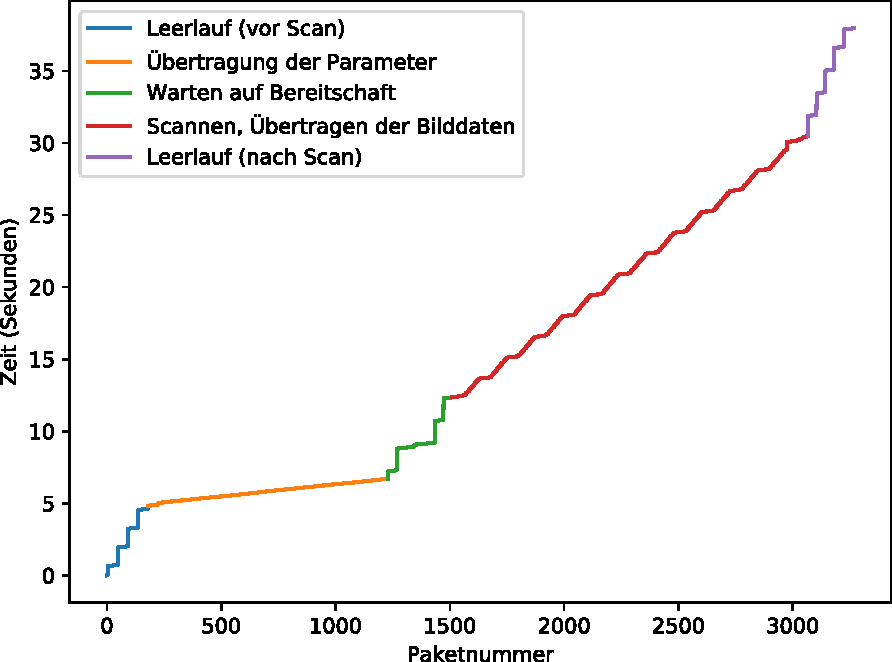
\includegraphics[height=7cm]{images/time_diagram.pdf}
  \end{figure}
  \begin{itemize}
    \item an bestimmten Stellen auf Bereitschaft des Geräts warten, sonst Absturz
  \end{itemize}
}

\frame{\frametitle{Funktion der jeweiligen Bytes}
\begin{itemize}
  \item Wie kann man ohne Dokumentation herausfinden, wie z.B. die Scanauflösung eingestellt werden kann?
  \item Zweimal scannen, nur diesen Parameter variieren
  \item Beispiel Auflösung, Abschnitt der übertragenen Bytefolge:
  \begin{itemize}
    \item 300 dpi:  \hspace{0.37cm} {\tt 000f\textcolor{red}{2c01}802004000100000001801000}
    \item 1200 dpi: \hspace{0.2cm} {\tt 000f\textcolor{red}{b004}802004000100000001801000}
  \end{itemize}
  \item nur wenige Parameter müssen verstanden werden, um das Gerät nutzbar zu machen
\end{itemize}
}

\frame{\frametitle{Bildverarbeitung}
  \begin{itemize}
    \item Helligkeitsunterschiede pro Spalte ausgleichen
    \begin{itemize}
      \item Helligkeit pro Spalte unterschiedlich
      \item Scanner nimmt Leerbild auf
      \item Ausgleichen: Division, nicht Subtraktion!
      \begin{figure}[H]
        \raggedright
        \begin{tabular}{llll}
        & 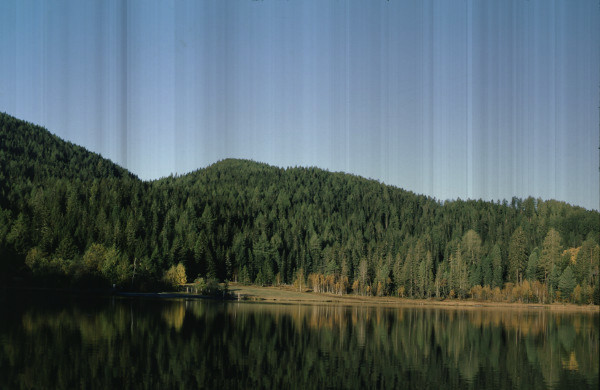
\includegraphics[height=2cm, align=c]{images/presentation/division_1.jpg} &
        $/$ &
        
\includegraphics[height=2cm, align=c]{images/presentation/division_2.jpg} \\
        & & & \\
        $=$ &
        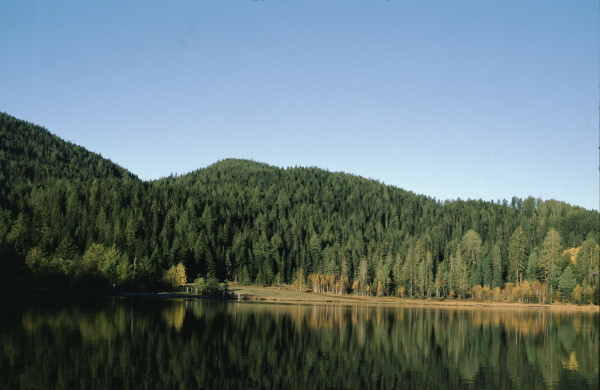
\includegraphics[height=2cm, align=c]{images/presentation/division_3.jpg} & & \\
        \end{tabular}
      \end{figure}
      
    \end{itemize}
    \item Gammakorrektur, Negativmaske, Wertebereich
    \item automatisches Zuschneiden
    
  \end{itemize}
}

\frame{\frametitle{Staub-/Kratzerkorrektur}
  \begin{figure}[H]
    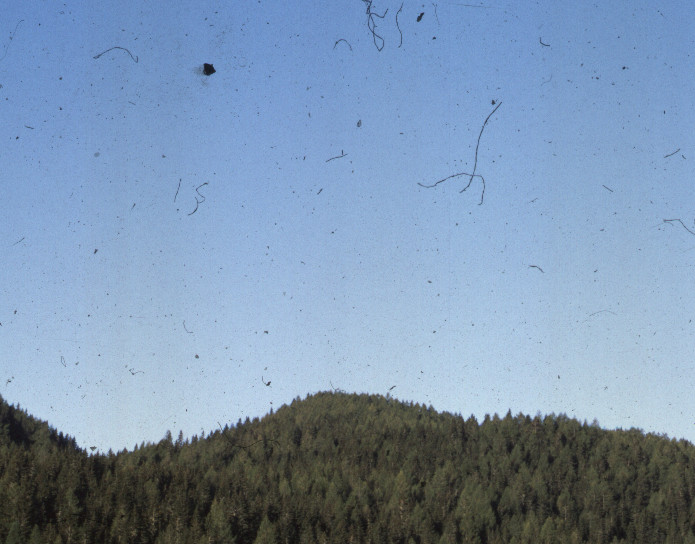
\includegraphics[height=4cm]{images/presentation/inpaint_1.jpg}
    \quad
    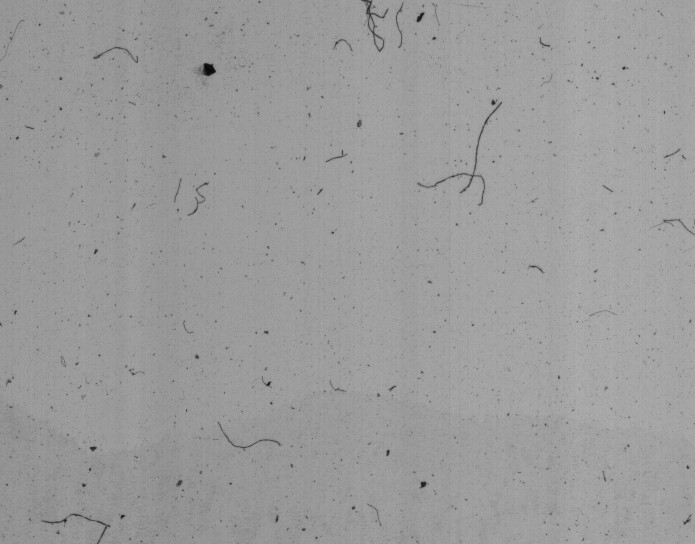
\includegraphics[height=4cm]{images/presentation/inpaint_2.jpg} \\
    \vspace{0.1cm}
    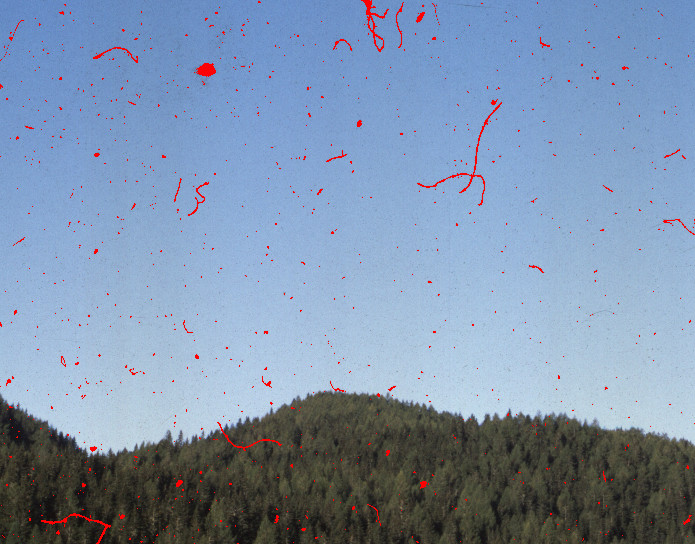
\includegraphics[height=4cm]{images/presentation/inpaint_3.jpg}
    \quad
    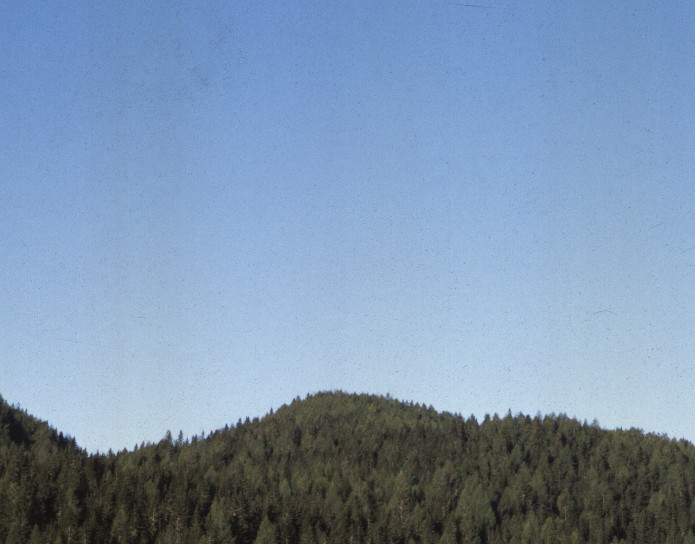
\includegraphics[height=4cm]{images/presentation/inpaint_4.jpg}
  \end{figure}
}

\frame{\frametitle{Ausblick: SANE}
  \begin{itemize}
    \item Linux-Scannerframework mit GUI und Client/Server
    \item hat Treiber für CrystalScan 7200, funktioniert aber nicht bei diesem Exemplar
    \item zumindest Grundfunktionen (Scannen mit einstellbarer Auflösung)
          in SANE nutzbar machen
  \end{itemize}
}

\frame{
  \usebeamerfont*{frametitle}\usebeamercolor[fg]{frametitle}
  \center{Live-Demo}
}

\end{document}
